\section{Evaluation}
To determine how well the system complies with criterion \ref{crit:cost} and \ref{crit:timesaving} of the solution criteria in \secref{chap:solutioncriteria} and how the system can alleviate the problem statement, we carry out an evaluation process. More specifically, we want to evaluate the following:
% What do we look at to evaluate?
\begin{itemize}
\item How accurately does the regression models reflect the actual traffic?
\item Does the routes found based on the regression models reflect reality?
\item Are routes found by the system, based on the regression models be faster than route chosen by drivers?
\end{itemize}
% How do we evaluate?
To answer the above questions, we consider the model accuracy and time savings of the routes. 

The model accuracy is the difference between the predicted traffic of the regression model and the actual traffic. In order to find the model accuracy we consider both the accuracy on a route basis as well as on an edge basis.

Time savings represents how much faster a found route is than an actual route. This is found by comparing actual routes from a test set of routes and routes found by querying the system the same start and destination.

\subsubsection{Route evaluation}
The following method is used to find the differences between real routes driven as given by the test-set and the routes found by the system.
\begin{enumerate}
\item First, we select a route $R=(n_1,...n_m)$ from the GPS data that originates in $n_1$ and ends in $n_m$. We then, directly from the data, determine weight of the route, $W_o(R)$.
\item Secondly, we compute a new weight, $W_{a}(R)$ for every edge $(n_i,n_{i+1}) \  for \  1 \leq i < m$ with the weight function described in Section \ref{sec:weight-function}.
\item Now, we traverse the road network to find a new route, $R'$ originating in $n_1$ and ending in $n_m$ such that the route is the shortest path (in time) from $n_1$ to $n_m$ by using the weight of each edge determined by the weight function.
\item We compare $W_o(R)$ and $W_a(R)$ to see the total weight difference. This is the \emph{route model accuracy}.
\item Finally, we compare $W_a(R')$ with $W_a(R)$ and find the difference. This is the \emph{time improvement}.
\end{enumerate}
The process is illustrated in the graphs in \figref{fig:eval}. Blue nodes represent start nodes, green nodes represent goal nodes where the number in goal nodes are the aggregate weight of all the edges in the route. 

Red arrows represents the uninformed route $R$, with a total weight of 7. $R$ with adjusted weights, has a total weight of 8. This means that the regression models has a route model accuracy of $\frac{7}{8}=0.875=87.5\%$. 

By computing the informed route $R'$, based on the regression model weights, the route marked with yellow arrows are found. $R'$ has a total weight of 6; a lower weight than $R$. This means that the time improvement is 1.

\begin{figure}
\centering
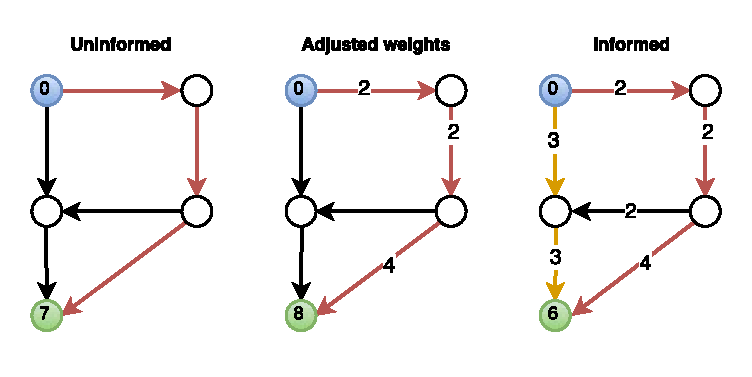
\includegraphics[width=\textwidth]{figures/eval.pdf}
\caption{The evaluation process}
\label{fig:eval}
\end{figure}

We follow the approach on a set of 10 fairly small routes that has no signs of intermediate stops, since intermediate stops in the route, without further measuers taken, would skewer the travel time in favor of our system. 
\begin{table}[]
\centering
\begin{tabular}{llllll}
\textbf{Route} & \textbf{$W_o(R)$} & \textbf{$W_a(R)$}  & \textbf{$W_a(R')$} & \textbf{RMA (\%)} & \textbf{TI (\%)} \\ \hline
$r_1$          & 1767              & 2572               & 1726               & 68.7                         & 32.9 \\
$r_2$          & 7023              & 4183               & 2574               & 59.6                         & 38.5 \\
$r_3$          & 2735              & 1793               & 1425               & 65.6                         & 20.5 \\
$r_4$          & 873               & 1010               & 855                & 86.4                         & 15.3 \\
$r_5$          & 5144              & 4915               & 2803               & 95.5                         & 43.0 \\
$r_6$          & 476               & 903                & 620                & 52.7                         & 31.3 \\
$r_7$          & 2432              & 2368               & 1770               & 97.3                         & 25.2 \\
$r_8$          & 2227              & 1431               & 1153               & 64.3                         & 19.4 \\
$r_9$          & 2991              & 13565              & 3250               & 22.0                         & 76.0 \\
$r_{10}$       & 1158              & 1153               & 1101               & 99.6                         & 4.51 \\ \hline
mean       	   &                   &                    &                    & 71.17                        & 30.661
\end{tabular}
\caption{RMA = Route Model Accuracy = $100 * \frac{min(W_o(R), W_a(R))}{max(W_o(R), W_a(R))}$\\
	     TI = Time Improvement = $100 * \frac{W_a(R) - W_a(R')}{W_a(R)}$}
\label{tab:eval-results}
\end{table}
Table \ref{tab:eval-results} shows the time in seconds, $W_0(R)$, for the uninformed route $R$,  the adjusted time, $W_a(R)$, for route $R$, and the informed time $W_a(R)$ for the new route, $R'$.

\emph{Route Model Accuracy } (\textbf{RMA}) represents the difference between the uninformed weight and the adjusted weight. The closer the route model accuracy is to 100, closer the regression models are to represent the actual traffic.
 
\emph{Time Improvement} (\textbf{TI}) represents the time saved for route $r_i$ by traveling the informed route instead of the uninformed route. The higher the time improvement, the better the informed routing is.

The mean route model accuracy of 71.17\%, shows that the regression models predicts the traffic within 71.17\% of the actual traffic. 

The mean value for \todo{kunne være rart at vide om det var underestimate / overestimate}time saved shows that for the tested routes, there are on average 30.661\% time saved by using the routes used by the route finding. However, it is worthwhile to note that it is not known if the drivers in the test routes was using some kind of GPS routing or not, which means that it is not possible to tell if the system outperforms routes selected by drivers or other systems.

However, the mean route model accuracy in \tabref{tab:eval-results} only shows the aggregate accuracy, which could be misleading if there is a high deviation in the regression model predictions and the actual traffic, throughout the edges. For this reason, the regression model accuracy must also be determined on an edge basis.

\subsubsection{Edge regression model}